\section{KLEE}

\subsection{Installation}

KLEE building from source is tricky.
Easiest way to use KLEE is to install docker\footnote{\url{https://docs.docker.com/engine/installation/linux/ubuntulinux/}} and then to run KLEE docker image\footnote{\url{http://klee.github.io/docker/}}.
The path where KLEE files residing can look like
\textbf{/var/lib/docker/aufs/mnt/(lots of hexadecimal digits)/home/klee}.

% subsections:
\input{KLEE/eq_EN.tex}
\subsection{Zebra puzzle (\ac{AKA} Einstein puzzle)}
\label{zebra_SMT}

Zebra puzzle is a popular puzzle, defined as follows:

% FIXME remove paragraph at first line
\begin{framed}
\begin{quotation}
1.There are five houses.\\
2.The Englishman lives in the red house.\\
3.The Spaniard owns the dog.\\
4.Coffee is drunk in the green house.\\
5.The Ukrainian drinks tea.\\
6.The green house is immediately to the right of the ivory house.\\
7.The Old Gold smoker owns snails.\\
8.Kools are smoked in the yellow house.\\
9.Milk is drunk in the middle house.\\
10.The Norwegian lives in the first house.\\
11.The man who smokes Chesterfields lives in the house next to the man with the fox.\\
12.Kools are smoked in the house next to the house where the horse is kept.\\
13.The Lucky Strike smoker drinks orange juice.\\
14.The Japanese smokes Parliaments.\\
15.The Norwegian lives next to the blue house.\\
\\
Now, who drinks water? Who owns the zebra?\\
\\
In the interest of clarity, it must be added that each of the five houses is painted a different color, and their inhabitants are of different national extractions, own different pets, drink different beverages and smoke different brands of American cigarets [sic]. One other thing: in statement 6, right means your right.
\end{quotation}
\end{framed}
( \url{https://en.wikipedia.org/wiki/Zebra_Puzzle} ) \\
\\
It's a very good example of \ac{CSP}.

We would encode each entity as integer variable, representing number of house.

Then, to define that Englishman lives in red house, we will add this constraint: \TT{Englishman == Red}, meaning that number of a house where Englishmen resides and which is painted in red is the same.

To define that Norwegian lives next to the blue house, we don't realy know, if it is at left side of blue house or at right side, but we know that house numbers are different by just 1.
So we will define this constraint: \TT{Norwegian==Blue-1 OR Norwegian==Blue+1}.

We will also need to limit all house numbers, so they will be in range of 1..5.

We will also use \TT{Distinct} to show that all various entities of the same type are all has different house numbers.

\lstinputlisting[style=custompy]{SMT/zebra.py}

When we run it, we got correct result:

\begin{lstlisting}
sat
[Snails = 3,
 Blue = 2,
 Ivory = 4,
 OrangeJuice = 4,
 Parliament = 5,
 Yellow = 1,
 Fox = 1,
 Zebra = 5,
 Horse = 2,
 Dog = 4,
 Tea = 2,
 Water = 1,
 Chesterfield = 2,
 Red = 3,
 Japanese = 5,
 LuckyStrike = 4,
 Norwegian = 1,
 Milk = 3,
 Kools = 1,
 OldGold = 3,
 Ukrainian = 2,
 Coffee = 5,
 Green = 5,
 Spaniard = 4,
 Englishman = 3]
\end{lstlisting}


\subsection{Sudoku puzzle}
\label{sudoku_SMT}

Sudoku puzzle is a 9*9 grid with some cells filled with values, some are empty:

% copypasted from http://www.texample.net/tikz/examples/sudoku/
\newcounter{row}
\newcounter{col}

\newcommand\setrow[9]{
  \setcounter{col}{1}
  \foreach \n in {#1, #2, #3, #4, #5, #6, #7, #8, #9} {
    \edef\x{\value{col} - 0.5}
    \edef\y{9.5 - \value{row}}
    \node[anchor=center] at (\x, \y) {\n};
    \stepcounter{col}
  }
  \stepcounter{row}
}

\begin{center}
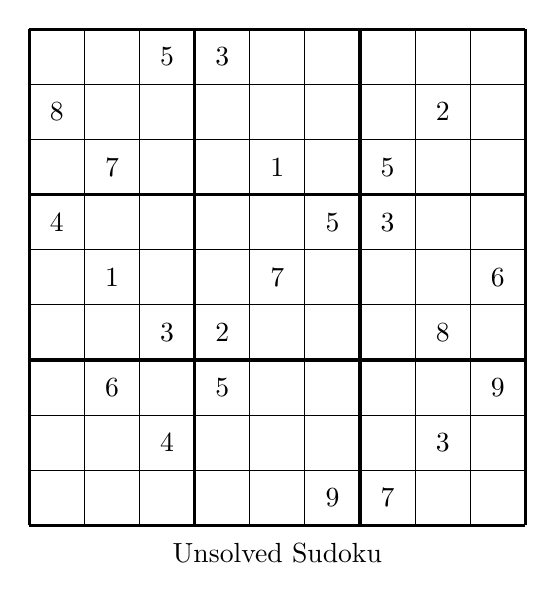
\begin{tikzpicture}[scale=.7]
  \begin{scope}
    \draw (0, 0) grid (9, 9);
    \draw[very thick, scale=3] (0, 0) grid (3, 3);

    \setcounter{row}{1}
    \setrow { }{ }{5}  {3}{ }{ }  { }{ }{ }
    \setrow {8}{ }{ }  { }{ }{ }  { }{2}{ }
    \setrow { }{7}{ }  { }{1}{ }  {5}{ }{ }

    \setrow {4}{ }{ }  { }{ }{5}  {3}{ }{ }
    \setrow { }{1}{ }  { }{7}{ }  { }{ }{6}
    \setrow { }{ }{3}  {2}{ }{ }  { }{8}{ }

    \setrow { }{6}{ }  {5}{ }{ }  { }{ }{9}
    \setrow { }{ }{4}  { }{ }{ }  { }{3}{ }
    \setrow { }{ }{ }  { }{ }{9}  {7}{ }{ }

    \node[anchor=center] at (4.5, -0.5) {Unsolved Sudoku};
  \end{scope}
\end{tikzpicture}
\end{center}

Numbers of each row must be unique, i.e., it must contain all 9 numbers in range of 1..9 without repetition.
Same story for each column and also for each 3*3 square.

This puzzle is good candidate to try \ac{SMT} solver on, because it's essentially an unsolved system of equations.

\subsubsection{The first idea}

The only thing we must decide is that how to determine in one expression, if the input 9 variables has all 9 unique numbers?
They are not ordered or sorted, after all.

From the school-level arithmetics, we can devise this idea:

\begin{equation}
\underbrace{10^{i_1} + 10^{i_2} + \cdots + 10^{i_9}}_9 = 1111111110
\end{equation}

Take each input variable, calculate $10^i$ and sum them all.
If all input values are unique, each will be settled at its own place.
Even more than that: there will be no holes, i.e., no skipped values.
So, in case of Sudoku, 1111111110 number will be final result, indicating that all 9 input values are unique, in range of 1..9.

Exponentiation is heavy operation, can we use binary operations? Yes, just replace 10 with 2:

\begin{equation}
\underbrace{2^{i_1} + 2^{i_2} + \cdots + 2^{i_9}}_9 = 1111111110_2
\end{equation}

The effect is just the same, but the final value is in base 2 instead of 10.

Now a working example:

\lstinputlisting{SMT/sudoku_plus.py}
( \url{https://github.com/DennisYurichev/SAT_SMT_article/blob/master/SMT/sudoku_plus.py} )

\begin{lstlisting}
% time python sudoku_plus.py
1 4 5 3 2 7 6 9 8
8 3 9 6 5 4 1 2 7
6 7 2 9 1 8 5 4 3
4 9 6 1 8 5 3 7 2
2 1 8 4 7 3 9 5 6
7 5 3 2 9 6 4 8 1
3 6 7 5 4 2 8 1 9
9 8 4 7 6 1 2 3 5
5 2 1 8 3 9 7 6 4

real    0m11.717s
user    0m10.896s
sys     0m0.068s
\end{lstlisting}

Even more, we can replace summing operation to logical OR:

\begin{equation}
\underbrace{2^{i_1} \vee 2^{i_2} \vee \cdots \vee 2^{i_9}}_9 = 1111111110_2
\end{equation}

% FIXME: только часть исходника
\lstinputlisting{SMT/sudoku_or.py}
( \url{https://github.com/DennisYurichev/SAT_SMT_article/blob/master/SMT/sudoku_or.py} )

Now it works much faster. Z3 handles OR operation over bit vectors better than addition?

\begin{lstlisting}
% time python sudoku_or.py
1 4 5 3 2 7 6 9 8
8 3 9 6 5 4 1 2 7
6 7 2 9 1 8 5 4 3
4 9 6 1 8 5 3 7 2
2 1 8 4 7 3 9 5 6
7 5 3 2 9 6 4 8 1
3 6 7 5 4 2 8 1 9
9 8 4 7 6 1 2 3 5
5 2 1 8 3 9 7 6 4

real    0m1.429s
user    0m1.393s
sys     0m0.036s
\end{lstlisting}

The puzzle I used as example is dubbed as one of the hardest known
\footnote{\url{http://www.mirror.co.uk/news/weird-news/worlds-hardest-sudoku-can-you-242294}} (well, for humans).
It took $\approx 1.4$ seconds on my Intel Core i3-3110M 2.4GHz notebook to solve it.

\subsubsection{The second idea}

My first approach is far from effective, I did what first came to my mind and worked.
Another approach is to use \TT{distinct} command from SMT-LIB, which tells Z3 that some variables must be distinct (or unique).
This command is also available in Z3 Python interface.

I've rewritten my first Sudoku solver, now it operates over \textit{Int} \textit{sort}, it has \TT{distinct} commands instead of bit operations,
and now also other constaint added: each cell value must be in 1..9 range, because, otherwise, Z3 will offer (although correct) solution with too big
and/or negative numbers.

% FIXME: только часть исходника
\lstinputlisting{SMT/sudoku2.py}
( \url{https://github.com/DennisYurichev/SAT_SMT_article/blob/master/SMT/sudoku2.py} )

\begin{lstlisting}
% time python sudoku2.py
1 4 5 3 2 7 6 9 8
8 3 9 6 5 4 1 2 7
6 7 2 9 1 8 5 4 3
4 9 6 1 8 5 3 7 2
2 1 8 4 7 3 9 5 6
7 5 3 2 9 6 4 8 1
3 6 7 5 4 2 8 1 9
9 8 4 7 6 1 2 3 5
5 2 1 8 3 9 7 6 4

real    0m0.382s
user    0m0.346s
sys     0m0.036s
\end{lstlisting}

That's much faster.

\subsubsection{Conclusion}

\ac{SMT}-solvers are so helpful, is that our Sudoku solver has nothing else, we have just defined relationships between variables (cells).

\subsubsection{Homework}

As it seems, true Sudoku puzzle is the one which has only one solution.
The piece of code I've included here shows only the first one.
Using the method described earlier (\ref{SMTEnumerate}, also called ``model counting''), 
try to find more solutions, or prove that the solution you have just found is the only one possible.

\subsubsection{Further reading}

\url{http://www.norvig.com/sudoku.html}

\subsubsection{Sudoku as a \ac{SAT} problem}

It's also possible to represend Sudoku puzzle as a huge \ac{CNF} equation and use \ac{SAT}-solver to find solution, but it's just trickier.

Some articles about it:
\textit{Building a Sudoku Solver with SAT}\footnote{\url{http://ocw.mit.edu/courses/electrical-engineering-and-computer-science/6-005-elements-of-software-construction-fall-2011/assignments/MIT6_005F11_ps4.pdf}},
Tjark Weber, \textit{A SAT-based Sudoku Solver}\footnote{\url{https://www.lri.fr/~conchon/mpri/weber.pdf}},
Ines Lynce, Joel Ouaknine, \textit{Sudoku as a SAT Problem}\footnote{\url{http://sat.inesc-id.pt/~ines/publications/aimath06.pdf}},
Gihwon Kwon, Himanshu Jain, \textit{Optimized CNF Encoding for Sudoku Puzzles}\footnote{\url{http://www.cs.cmu.edu/~hjain/papers/sudoku-as-SAT.pdf}}.

\ac{SMT}-solver can also use \ac{SAT}-solver in its core, so it does all mundane translating work.
As a ``compiler'', it may not do this in the most efficient way, though.


\section{Unit test: HTML/CSS color}

The most popular ways to represent HTML/CSS color is by English name (e.g., ``red'') and by 6-digit hexadecimal number (e.g., ``\#0077CC'').
There is third, less popular way: if each byte in hexadecimal number has two doubling digits, it can be \textit{abbreviated}, thus, 
``\#0077CC'' can be written just as ``\#07C''.

Let's write a function to convert 3 color components into name (if possible, first priority), 3-digit hexadecimal form (if possible, second priority),
or as 6-digit hexadecimal form (as a last resort).

\lstinputlisting{KLEE/color.c}

There are 5 possible paths in function, and let's see, if KLEE could find them all?
It's indeed so:

\begin{lstlisting}
% clang -emit-llvm -c -g color.c

% klee color.bc
KLEE: output directory is "/home/klee/klee-out-134"
KLEE: WARNING: undefined reference to function: sprintf
KLEE: WARNING: undefined reference to function: strcpy
KLEE: WARNING ONCE: calling external: strcpy(51867584, 51598960)
KLEE: ERROR: /home/klee/color.c:33: external call with symbolic argument: sprintf
KLEE: NOTE: now ignoring this error at this location
KLEE: ERROR: /home/klee/color.c:28: external call with symbolic argument: sprintf
KLEE: NOTE: now ignoring this error at this location

KLEE: done: total instructions = 479
KLEE: done: completed paths = 19
KLEE: done: generated tests = 5
\end{lstlisting}

We can ignore calls to strcpy() and sprintf(), because we are not really interesting in state of \TT{out} variable.

So there are exactly 5 paths:

\begin{lstlisting}
% ls klee-last
assembly.ll   run.stats            test000003.ktest     test000005.ktest
info          test000001.ktest     test000003.pc        test000005.pc
messages.txt  test000002.ktest     test000004.ktest     warnings.txt
run.istats    test000003.exec.err  test000005.exec.err
\end{lstlisting}

1st set of input variables will result in ``red'' string:

\begin{lstlisting}
% ktest-tool --write-ints klee-last/test000001.ktest
ktest file : 'klee-last/test000001.ktest'
args       : ['color.bc']
num objects: 3
object    0: name: b'R'
object    0: size: 1
object    0: data: b'\xff'
object    1: name: b'G'
object    1: size: 1
object    1: data: b'\x00'
object    2: name: b'B'
object    2: size: 1
object    2: data: b'\x00'
\end{lstlisting}

2nd set of input variables will result in ``green'' string:

\begin{lstlisting}
% ktest-tool --write-ints klee-last/test000002.ktest
ktest file : 'klee-last/test000002.ktest'
args       : ['color.bc']
num objects: 3
object    0: name: b'R'
object    0: size: 1
object    0: data: b'\x00'
object    1: name: b'G'
object    1: size: 1
object    1: data: b'\xff'
object    2: name: b'B'
object    2: size: 1
object    2: data: b'\x00'
\end{lstlisting}

3rd set of input variables will result in ``\#010000'' string:

\begin{lstlisting}
% ktest-tool --write-ints klee-last/test000003.ktest
ktest file : 'klee-last/test000003.ktest'
args       : ['color.bc']
num objects: 3
object    0: name: b'R'
object    0: size: 1
object    0: data: b'\x01'
object    1: name: b'G'
object    1: size: 1
object    1: data: b'\x00'
object    2: name: b'B'
object    2: size: 1
object    2: data: b'\x00'
\end{lstlisting}

4th set of input variables will result in ``blue'' string:

\begin{lstlisting}
% ktest-tool --write-ints klee-last/test000004.ktest
ktest file : 'klee-last/test000004.ktest'
args       : ['color.bc']
num objects: 3
object    0: name: b'R'
object    0: size: 1
object    0: data: b'\x00'
object    1: name: b'G'
object    1: size: 1
object    1: data: b'\x00'
object    2: name: b'B'
object    2: size: 1
object    2: data: b'\xff'
\end{lstlisting}

5th set of input variables will result in ``\#F01'' string:

\begin{lstlisting}
% ktest-tool --write-ints klee-last/test000005.ktest
ktest file : 'klee-last/test000005.ktest'
args       : ['color.bc']
num objects: 3
object    0: name: b'R'
object    0: size: 1
object    0: data: b'\xff'
object    1: name: b'G'
object    1: size: 1
object    1: data: b'\x00'
object    2: name: b'B'
object    2: size: 1
object    2: data: b'\x11'
\end{lstlisting}

These 5 sets of input variables can form a unit test for our function.


\section{Unit test: strcmp() function}

The standard \TT{strcmp()} function from C library can return 0, -1 or 1, depending of comparison result.

Here is my own implementation of \TT{strcmp()}:

\lstinputlisting{KLEE/strcmp.c}

Let's find out, if KLEE is capable of finding all three paths?
I intentionaly made things simpler for KLEE by limiting input arrays to two 2 bytes or to 1 character + terminal zero byte.

\begin{lstlisting}
% clang -emit-llvm -c -g strcmp.c

% klee strcmp.bc
KLEE: output directory is "/home/klee/klee-out-131"
KLEE: ERROR: /home/klee/strcmp.c:35: invalid klee_assume call (provably false)
KLEE: NOTE: now ignoring this error at this location
KLEE: ERROR: /home/klee/strcmp.c:36: invalid klee_assume call (provably false)
KLEE: NOTE: now ignoring this error at this location

KLEE: done: total instructions = 137
KLEE: done: completed paths = 5
KLEE: done: generated tests = 5

% ls klee-last
assembly.ll   run.stats            test000002.ktest     test000004.ktest
info          test000001.ktest     test000002.pc        test000005.ktest
messages.txt  test000001.pc        test000002.user.err  warnings.txt
run.istats    test000001.user.err  test000003.ktest
\end{lstlisting}

The first two errors are about \TT{klee\_assume()}.
These are input values on which \TT{klee\_assume()} calls are stuck.
We can ignore them, or take a peek out of curiosity:

\begin{lstlisting}
% ktest-tool --write-ints klee-last/test000001.ktest
ktest file : 'klee-last/test000001.ktest'
args       : ['strcmp.bc']
num objects: 2
object    0: name: b'input1'
object    0: size: 2
object    0: data: b'\x00\x00'
object    1: name: b'input2'
object    1: size: 2
object    1: data: b'\x00\x00'

% ktest-tool --write-ints klee-last/test000002.ktest
ktest file : 'klee-last/test000002.ktest'
args       : ['strcmp.bc']
num objects: 2
object    0: name: b'input1'
object    0: size: 2
object    0: data: b'a\xff'
object    1: name: b'input2'
object    1: size: 2
object    1: data: b'\x00\x00'
\end{lstlisting}

Three rest files are the input values for each path inside of my implementation of \TT{strcmp()}:

\begin{lstlisting}
% ktest-tool --write-ints klee-last/test000003.ktest
ktest file : 'klee-last/test000003.ktest'
args       : ['strcmp.bc']
num objects: 2
object    0: name: b'input1'
object    0: size: 2
object    0: data: b'b\x00'
object    1: name: b'input2'
object    1: size: 2
object    1: data: b'c\x00'

% ktest-tool --write-ints klee-last/test000004.ktest
ktest file : 'klee-last/test000004.ktest'
args       : ['strcmp.bc']
num objects: 2
object    0: name: b'input1'
object    0: size: 2
object    0: data: b'c\x00'
object    1: name: b'input2'
object    1: size: 2
object    1: data: b'a\x00'

% ktest-tool --write-ints klee-last/test000005.ktest
ktest file : 'klee-last/test000005.ktest'
args       : ['strcmp.bc']
num objects: 2
object    0: name: b'input1'
object    0: size: 2
object    0: data: b'a\x00'
object    1: name: b'input2'
object    1: size: 2
object    1: data: b'a\x00'
\end{lstlisting}

3rd is about first argument (``b'') is lesser than the second (``c'').
4th is opposite (``c'' and ``a'').
5th is when they are equal (``a'' and ``a'').

Using these 3 test cases, we've got full coverage of our implementation of \TT{strcmp()}.


\section{UNIX date/time}

UNIX date/time\footnote{\url{https://en.wikipedia.org/wiki/Unix_time}} is a number of seconds that have elapsed since 1-Jan-1970 00:00 UTC.
C/C++ gmtime() function is used to decode this value into human-readable date/time.

Here is a piece of code I've copypasted from some ancient version of Minix OS 
(\url{http://www.cise.ufl.edu/~cop4600/cgi-bin/lxr/http/source.cgi/lib/ansi/gmtime.c}) and reworked slightly:

\lstinputlisting[numbers=left]{KLEE/klee_time1.c}

Let's try it:

\begin{lstlisting}
% clang -emit-llvm -c -g klee_time1.c
...

% klee klee_time1.bc
KLEE: output directory is "/home/klee/klee-out-107"
KLEE: WARNING: undefined reference to function: printf
KLEE: ERROR: /home/klee/klee_time1.c:86: external call with symbolic argument: printf
KLEE: NOTE: now ignoring this error at this location
KLEE: ERROR: /home/klee/klee_time1.c:83: ASSERTION FAIL: 0
KLEE: NOTE: now ignoring this error at this location

KLEE: done: total instructions = 101579
KLEE: done: completed paths = 1635
KLEE: done: generated tests = 2
\end{lstlisting}

Wow, assert() at line 83 has been triggered, why?
Let's see a value of UNIX time which triggers it:

\begin{lstlisting}
% ls klee-last | grep err
test000001.exec.err
test000002.assert.err

% ktest-tool --write-ints klee-last/test000002.ktest
ktest file : 'klee-last/test000002.ktest'
args       : ['klee_time1.bc']
num objects: 1
object    0: name: b'time'
object    0: size: 4
object    0: data: 978278400
\end{lstlisting}

Let's decode this value using UNIX date utility:

\begin{lstlisting}
% date -u --date='@978278400'
Sun Dec 31 16:00:00 UTC 2000
\end{lstlisting}

After my investigation, I've found that \TT{month} variable can hold incorrect value of 12 (while 11 is maximal, for December), 
because LEAPYEAR() macro should receive year number as 2000, not as 100.
So I've introduced a bug during rewritting this function, and KLEE found it!

Just interesting, what would be if I'll replace switch() to array of strings, like it usually happens in concise C/C++ code?

\begin{lstlisting}
	...

const char *_months[] =
{
	"January", "February", "March",
	"April", "May", "June",
	"July", "August", "September",
	"October", "November", "December"
};

	...

	while (dayno >= _ytab[LEAPYEAR(year)][month])
	{
		dayno -= _ytab[LEAPYEAR(year)][month];
		month++;
	}
	
	char *s=_months[month];

	printf ("%04d-%s-%02d %02d:%02d:%02d\n", YEAR0+year, s, dayno+1, hour, minutes, seconds);
	printf ("week day: %s\n", _days[wday]);	
	
	...

\end{lstlisting}

KLEE detects attempt to read beyond array boundaries:

\begin{lstlisting}
% klee klee_time2.bc
KLEE: output directory is "/home/klee/klee-out-108"
KLEE: WARNING: undefined reference to function: printf
KLEE: ERROR: /home/klee/klee_time2.c:69: external call with symbolic argument: printf
KLEE: NOTE: now ignoring this error at this location
KLEE: ERROR: /home/klee/klee_time2.c:67: memory error: out of bound pointer
KLEE: NOTE: now ignoring this error at this location

KLEE: done: total instructions = 101716
KLEE: done: completed paths = 1635
KLEE: done: generated tests = 2
\end{lstlisting}

This is the same UNIX time value we've already seen:

\begin{lstlisting}
% ls klee-last | grep err
test000001.exec.err
test000002.ptr.err

% ktest-tool --write-ints klee-last/test000002.ktest
ktest file : 'klee-last/test000002.ktest'
args       : ['klee_time2.bc']
num objects: 1
object    0: name: b'time'
object    0: size: 4
object    0: data: 978278400
\end{lstlisting}

So, if this piece of code can be triggered on remote computer, with this input value (\emph{input of death}),
it's possible to crash the process (with some luck, though).\\
\\
OK, now I'm fixing a bug by moving year subtracting expression to line 43, and let's find, what UNIX time value corresponds to some fancy date
like 2022-February-2?

\lstinputlisting[numbers=left]{KLEE/klee_time3.c}

\begin{lstlisting}
% clang -emit-llvm -c -g klee_time3.c
...

% klee klee_time3.bc
KLEE: output directory is "/home/klee/klee-out-109"
KLEE: WARNING: undefined reference to function: klee_assert
KLEE: WARNING ONCE: calling external: klee_assert(0)
KLEE: ERROR: /home/klee/klee_time3.c:47: failed external call: klee_assert
KLEE: NOTE: now ignoring this error at this location

KLEE: done: total instructions = 101087
KLEE: done: completed paths = 1635
KLEE: done: generated tests = 1635

% ls klee-last | grep err
test000587.external.err

% ktest-tool --write-ints klee-last/test000587.ktest
ktest file : 'klee-last/test000587.ktest'
args       : ['klee_time3.bc']
num objects: 1
object    0: name: b'time'
object    0: size: 4
object    0: data: 1645488640

% date -u --date='@1645488640'
Tue Feb 22 00:10:40 UTC 2022
\end{lstlisting}

Success, but hours/minutes/seconds are seems random---they are random indeed, because, KLEE satisfied all constraints we've put, nothing else.
We didn't ask it to set hours/minutes/seconds to zeroes.

Let's add constraints to hours/minutes/seconds as well:

\begin{lstlisting}
	...

	if (YEAR0+year==2022 && month==1 && dayno+1==22 && hour==22 && minutes==22 && seconds==22)
		klee_assert(0);
	
	...
\end{lstlisting}

Let's run it and check \dots

\begin{lstlisting}
% ktest-tool --write-ints klee-last/test000597.ktest
ktest file : 'klee-last/test000597.ktest'
args       : ['klee_time3.bc']
num objects: 1
object    0: name: b'time'
object    0: size: 4
object    0: data: 1645568542

% date -u --date='@1645568542'
Tue Feb 22 22:22:22 UTC 2022
\end{lstlisting}

Now that is precise.

Yes, of course, C/C++ libraries has function(s) to encode human-readable date into UNIX time value, but what we've got here is KLEE working
\emph{antipode} of decoding function, \emph{inverse function} in a way.


\section{Inverse function for base64 decoder}

It's piece of cake for KLEE to reconstruct input base64 string given just base64 decoder code without corresponding encoder code.
I've copypasted this piece of code from
\url{http://www.opensource.apple.com/source/QuickTimeStreamingServer/QuickTimeStreamingServer-452/CommonUtilitiesLib/base64.c}.

We add constraints (lines 84, 85) so that output buffer must have byte values from 0 to 15.
We also tell to KLEE that the Base64decode() function must return 16 (i.e., size of output buffer in bytes, line 82).

\lstinputlisting[numbers=left]{KLEE/klee_base64.c}

\begin{lstlisting}
% clang -emit-llvm -c -g klee_base64.c
...

% klee klee_base64.bc
KLEE: output directory is "/home/klee/klee-out-99"
KLEE: WARNING: undefined reference to function: klee_assert
KLEE: ERROR: /home/klee/klee_base64.c:99: invalid klee_assume call (provably false)
KLEE: NOTE: now ignoring this error at this location
KLEE: WARNING ONCE: calling external: klee_assert(0)
KLEE: ERROR: /home/klee/klee_base64.c:104: failed external call: klee_assert
KLEE: NOTE: now ignoring this error at this location
KLEE: ERROR: /home/klee/klee_base64.c:85: memory error: out of bound pointer
KLEE: NOTE: now ignoring this error at this location
KLEE: ERROR: /home/klee/klee_base64.c:81: memory error: out of bound pointer
KLEE: NOTE: now ignoring this error at this location
KLEE: ERROR: /home/klee/klee_base64.c:65: memory error: out of bound pointer
KLEE: NOTE: now ignoring this error at this location

...
\end{lstlisting}

We're interesting in the second error, where \TT{klee\_assert()} has been triggered:

\begin{lstlisting}
% ls klee-last | grep err
test000001.user.err
test000002.external.err
test000003.ptr.err
test000004.ptr.err
test000005.ptr.err

% ktest-tool --write-ints klee-last/test000002.ktest
ktest file : 'klee-last/test000002.ktest'
args       : ['klee_base64.bc']
num objects: 1
object    0: name: b'input'
object    0: size: 32
object    0: data: b'AAECAwQFBgcICQoLDA0OD4\x00\xff\xff\xff\xff\xff\xff\xff\xff\x00'
\end{lstlisting}

This is indeed a real base64 string, terminated with the zero byte, just as it's requested by C/C++ standards.
The final zero byte at 31th byte (starting at zeroth byte) is our deed: so that KLEE would report lesser number of errors. % FIXME spelling

The base64 string is indeed correct:

\begin{lstlisting}
% echo AAECAwQFBgcICQoLDA0OD4 | base64 -d | hexdump -C
base64: invalid input
00000000  00 01 02 03 04 05 06 07  08 09 0a 0b 0c 0d 0e 0f  |................|
00000010
\end{lstlisting}

base64 decoder Linux utility I've just run blaming for ``invalid input''---it means the input string is not properly padded.
Now let's pad it manually, and decoder utility will no complain anymore:

\begin{lstlisting}
% echo AAECAwQFBgcICQoLDA0OD4== | base64 -d | hexdump -C
00000000  00 01 02 03 04 05 06 07  08 09 0a 0b 0c 0d 0e 0f  |................|
00000010
\end{lstlisting}

The reason our generated base64 string is not padded is because base64 decoders are usually discards padding symbols (``='') at the end.
In other words, they are not require them, so is the case of our decoder.
Hence, padding symbols are left unnoticed to KLEE.

So we again made \emph{antipode} or \emph{inverse function} of base64 decoder.


\input{KLEE/CRC_EN.tex}
\section{LZSS decompressor}

I've googled for a very simple \ac{LZSS} decompressor and landed at this page:
\url{http://www.opensource.apple.com/source/boot/boot-132/i386/boot2/lzss.c}.

Let's pretend, we're looking at unknown compressing algorithm with no compressor available.
Will it be possible to reconstruct a compressed piece of data so that decompressor would generate data we need?

Here is my first experiment:

\lstinputlisting{KLEE/klee_lzss1.c}

What I did is changing size of ring buffer from 4096 to 32, because if bigger, KLEE consumes all \ac{RAM} it can.
But I've found that KLEE can live with that small buffer.
I've also decreased \TT{COMPRESSED\_LEN} gradually to check, whether KLEE would find compressed piece of data, and it did:

% FIXME:
\begin{lstlisting}
% clang -emit-llvm -c -g klee_lzss.c
...

% time klee klee_lzss.bc
KLEE: output directory is "/home/klee/klee-out-7"
KLEE: WARNING: undefined reference to function: klee_assert
KLEE: ERROR: /home/klee/klee_lzss.c:122: invalid klee_assume call (provably false)
KLEE: NOTE: now ignoring this error at this location
KLEE: ERROR: /home/klee/klee_lzss.c:47: memory error: out of bound pointer
KLEE: NOTE: now ignoring this error at this location
KLEE: ERROR: /home/klee/klee_lzss.c:37: memory error: out of bound pointer
KLEE: NOTE: now ignoring this error at this location
KLEE: WARNING ONCE: calling external: klee_assert(0)
KLEE: ERROR: /home/klee/klee_lzss.c:124: failed external call: klee_assert
KLEE: NOTE: now ignoring this error at this location

KLEE: done: total instructions = 41417919
KLEE: done: completed paths = 437820
KLEE: done: generated tests = 4

real    13m0.215s
user    11m57.517s
sys     1m2.187s

% ls klee-last | grep err
test000001.user.err
test000002.ptr.err
test000003.ptr.err
test000004.external.err

% ktest-tool --write-ints klee-last/test000004.ktest
ktest file : 'klee-last/test000004.ktest'
args       : ['klee_lzss.bc']
num objects: 1
object    0: name: b'input'
object    0: size: 15
object    0: data: b'\xffBuffalo \x01b\x0f\x03\r\x05'
\end{lstlisting}

KLEE consumed $\approx 1GB$ of RAM and worked for $\approx 15$ minutes (on my Intel Core i3-3110M 2.4GHz notebook), 
but here it is, a 15 bytes which, if decompressed by our copypasted algorithm, will result in desired text!

During my experimentation, I've found that KLEE can do even more cooler thing, to find out size of compressed piece of data:

\begin{lstlisting}
int main()
{
	uint8_t input[24];
	uint8_t plain[24];
	uint32_t size;
  
	klee_make_symbolic(input, sizeof input, "input");
	klee_make_symbolic(&size, sizeof size, "size");
	
	decompress_lzss(plain, input, size);

	for (int i=0; i<23; i++)
		klee_assume (plain[i]=="Buffalo buffalo Buffalo"[i]);

	klee_assert(0);
	
	return 0;
}
\end{lstlisting}

\dots but then KLEE works much slower, consumes much more RAM and I had success only with even smaller pieces of desired text.

So how \ac{LZSS} works? Without peeking into Wikipedia, we can say that: 
if \ac{LZSS} compressor observes some data it already had, it replaces the data with a link to some place in past with size. 
If it observes something yet unseen, it puts data as is.
This is theory.
This is indeed what we've got. Desired text is three ``Buffalo'' words, the first and the last are equivalent, but the second is \emph{almost} equivalent, 
differing with first by one character.

That's what we see:

% FIXME: colored Buffalo, ``b'', slashes
\begin{lstlisting}
'\xffBuffalo \x01b\x0f\x03\r\x05'
\end{lstlisting}

Here is some control byte (0xff), ``Buffalo'' word is placed \emph{as is}, then another control byte (0x01), 
then we see beginning of the second word (``b'') and more
control bytes, perhaps, links to the beginning of the buffer.
These are command to decompressor, like, in plain English, ``copy data from the buffer we've already done, from that place to that place'', etc.

Interesting, is it possible to meddle into this piece of compressed data?
Out of whim, can we force KLEE to find a compressed data, where not just ``b'' character has been placed \emph{as is},
but also the second character of the word, i.e., ``bu''?

I've modified main() function by adding \TT{klee\_assume()}: now the 11th byte of input (compressed) data (right after ``b'' byte) must have ``u''.
I has no luck with 15 byte of compressed data, so I increased it to 16 bytes:

\begin{lstlisting}
int main()
{
#define COMPRESSED_LEN 16
	uint8_t input[COMPRESSED_LEN];
	uint8_t plain[24];
	uint32_t size=COMPRESSED_LEN;
  
	klee_make_symbolic(input, sizeof input, "input");
	
	klee_assume(input[11]=='u');
	
	decompress_lzss(plain, input, size);

	for (int i=0; i<23; i++)
		klee_assume (plain[i]=="Buffalo buffalo Buffalo"[i]);

	klee_assert(0);
	
	return 0;
}
\end{lstlisting}

\dots and voilà: KLEE found a compressed piece of data which satisfied our whimsical constraint:

\begin{lstlisting}
% time klee klee_lzss.bc
KLEE: output directory is "/home/klee/klee-out-9"
KLEE: WARNING: undefined reference to function: klee_assert
KLEE: ERROR: /home/klee/klee_lzss.c:97: invalid klee_assume call (provably false)
KLEE: NOTE: now ignoring this error at this location
KLEE: ERROR: /home/klee/klee_lzss.c:47: memory error: out of bound pointer
KLEE: NOTE: now ignoring this error at this location
KLEE: ERROR: /home/klee/klee_lzss.c:37: memory error: out of bound pointer
KLEE: NOTE: now ignoring this error at this location
KLEE: WARNING ONCE: calling external: klee_assert(0)
KLEE: ERROR: /home/klee/klee_lzss.c:99: failed external call: klee_assert
KLEE: NOTE: now ignoring this error at this location

KLEE: done: total instructions = 36700587
KLEE: done: completed paths = 369756
KLEE: done: generated tests = 4

real    12m16.983s
user    11m17.492s
sys     0m58.358s

% ktest-tool --write-ints klee-last/test000004.ktest
ktest file : 'klee-last/test000004.ktest'
args       : ['klee_lzss.bc']
num objects: 1
object    0: name: b'input'
object    0: size: 16
object    0: data: b'\xffBuffalo \x13bu\x10\x02\r\x05'
\end{lstlisting}

So now we find a piece of compressed data where two strings are placed \emph{as is}: ``Buffalo'' and ``bu''.

% FIXME: colored Buffalo and bu
\begin{lstlisting}
'\xffBuffalo \x13bu\x10\x02\r\x05'
\end{lstlisting}

Both pieces of compressed data, if feeded into our copypasted function, produce ``Buffalo buffalo Buffalo'' text string.

Please note, I still have no access to \ac{LZSS} compressor code, and I didn't get into \ac{LZSS} decompressor details yet.

Unfortunately, things are not that cool: 
KLEE is very slow and I had success only with small pieces of text, and also ring buffer size had to be decreased significantly
(original \ac{LZSS} decompressor with ring buffer of 4096 bytes cannot decompress correctly what we found).

Nevertheless, it's very impressive, taking into account the fact that we're not getting into internals of this specific LZSS decompressor.
Once more time, we've created \emph{antipode} of decompressor, or \emph{inverse function}.

Also, as it seems, KLEE isn't very good so far with decompression algorithms (but who's good then?).
I've also tried various JPEG/PNG/GIF decoders (which, of course, has decompressors), starting with simplest possible, and KLEE had stuck.


\subsection{strtodx() from RetroBSD}

Just found this function in RetroBSD:
\url{https://github.com/RetroBSD/retrobsd/blob/master/src/libc/stdlib/strtod.c}.
It converts a string into floating point number for given radix.

\lstinputlisting[numbers=left]{KLEE/strtodx.c}
( \url{https://github.com/DennisYurichev/SAT_SMT_by_example/blob/master/KLEE/strtodx.c} )

Interestinly, KLEE cannot handle floating-point arithmetic, but nevertheless, found something:

\begin{lstlisting}
...

KLEE: ERROR: /home/klee/klee_test.c:202: memory error: out of bound pointer

...

% ktest-tool klee-last/test003483.ktest
ktest file : 'klee-last/test003483.ktest'
args       : ['klee_test.bc']
num objects: 1
object    0: name: b'buf'
object    0: size: 10
object    0: data: b'-.0E-66\x00\x00\x00'
\end{lstlisting}

As it seems, string ``-.0E-66'' makes out of bounds array access (read) at line 202.
While further investigation, I've found that \TT{powersOf10[]} array is too short:
6th element (started at 0th) has been accessed.
And here we see part of array commented (line 79)!
Probably someone's mistake?


\subsection{Unit testing: simple expression evaluator (calculator)}

I has been looking for simple expression evaluator (calculator in other words) which takes expression like ``2+2'' on input and gives answer.
I've found one at \url{http://stackoverflow.com/a/13895198}.
Unfortunately, it has no bugs, so I've introduced one: a token buffer (\TT{buf[]} at line 31) is smaller than input buffer (\TT{input[]} at line 19).

\lstinputlisting[numbers=left,style=customc]{KLEE/calc.c}
( \url{https://github.com/DennisYurichev/SAT_SMT_by_example/blob/master/KLEE/calc.c} )

KLEE found buffer overflow with little effort (65 zero digits + one tabulation symbol):

\begin{lstlisting}
% ktest-tool --write-ints klee-last/test000468.ktest
ktest file : 'klee-last/test000468.ktest'
args       : ['calc.bc']
num objects: 1
object    0: name: b'input'
object    0: size: 128
object    0: data: b'0\t0000000000000000000000000000000000000000000000000000000000000000\xff\xff\xff\xff\xff\xff\xff\xff\xff\xff\xff\xff\xff\xff\xff\xff\xff\xff\xff\xff\xff\xff\xff\xff\xff\xff\xff\xff\xff\xff\xff\xff\xff\xff\xff\xff\xff\xff\xff\xff\xff\xff\xff\xff\xff\xff\xff\xff\xff\xff\xff\xff\xff\xff\xff\xff\xff\xff\xff\xff\xff\xff'
\end{lstlisting}

Hard to say, how tabulation symbol (\TT{\textbackslash{}t}) got into input[] array, but KLEE achieved what has been desired: buffer overflown.\\
\\
KLEE also found two expression strings which leads to division error (``0/0'' and ``0\%0''):

\begin{lstlisting}
% ktest-tool --write-ints klee-last/test000326.ktest
ktest file : 'klee-last/test000326.ktest'
args       : ['calc.bc']
num objects: 1
object    0: name: b'input'
object    0: size: 128
object    0: data: b'0/0\x00\xff\xff\xff\xff\xff\xff\xff\xff\xff\xff\xff\xff\xff\xff\xff\xff\xff\xff\xff\xff\xff\xff\xff\xff\xff\xff\xff\xff\xff\xff\xff\xff\xff\xff\xff\xff\xff\xff\xff\xff\xff\xff\xff\xff\xff\xff\xff\xff\xff\xff\xff\xff\xff\xff\xff\xff\xff\xff\xff\xff\xff\xff\xff\xff\xff\xff\xff\xff\xff\xff\xff\xff\xff\xff\xff\xff\xff\xff\xff\xff\xff\xff\xff\xff\xff\xff\xff\xff\xff\xff\xff\xff\xff\xff\xff\xff\xff\xff\xff\xff\xff\xff\xff\xff\xff\xff\xff\xff\xff\xff\xff\xff\xff\xff\xff\xff\xff\xff\xff\xff\xff\xff\xff\xff'

% ktest-tool --write-ints klee-last/test000557.ktest
ktest file : 'klee-last/test000557.ktest'
args       : ['calc.bc']
num objects: 1
object    0: name: b'input'
object    0: size: 128
object    0: data: b'0%0\x00\xff\xff\xff\xff\xff\xff\xff\xff\xff\xff\xff\xff\xff\xff\xff\xff\xff\xff\xff\xff\xff\xff\xff\xff\xff\xff\xff\xff\xff\xff\xff\xff\xff\xff\xff\xff\xff\xff\xff\xff\xff\xff\xff\xff\xff\xff\xff\xff\xff\xff\xff\xff\xff\xff\xff\xff\xff\xff\xff\xff\xff\xff\xff\xff\xff\xff\xff\xff\xff\xff\xff\xff\xff\xff\xff\xff\xff\xff\xff\xff\xff\xff\xff\xff\xff\xff\xff\xff\xff\xff\xff\xff\xff\xff\xff\xff\xff\xff\xff\xff\xff\xff\xff\xff\xff\xff\xff\xff\xff\xff\xff\xff\xff\xff\xff\xff\xff\xff\xff\xff\xff\xff\xff\xff'
\end{lstlisting}

Maybe this is not impressive result, nevertheless,
it's yet another reminder that division and remainder operations must be wrapped somehow in production code to avoid possible crash.


\input{KLEE/regexp_EN.tex}

\subsection{More examples}

\url{https://feliam.wordpress.com/2010/10/07/the-symbolic-maze/}

\subsection{Exercise}

Here is my crackme/keygenme, which may be tricky, but easy to solve using KLEE:
\url{http://challenges.re/74/}.


